% -*- latex -*-

\documentclass{acmsiggraph}

\usepackage[usenames]{color}
\definecolor{Red}{rgb}{1,0,0}
%\newcommand{\sticky}[1]{\textcolor{Red}{[#1]}}
\newcommand{\sticky}[1]{}

% This package apparently is for using Type 1 typefaces.
\usepackage{mathptmx}

\usepackage{graphicx}
\usepackage{varioref}
\usepackage{hyperref}

%% If you are submitting a paper to the annual conference, please replace 
%% the value ``0'' below with your OnlineID. If you are not submitting this
%% paper to the annual conference, you may safely leave it at ``0;'' it 
%% will not be included in the output.
% Since I am submitting this to PVG, not SIGGRAPH, I assume 0 is ok.
\onlineid{0}

% I don't know what these do; they are not documented, but I just copied
% them out of an example.
\acmcategory{Research}
\acmformat{print}

\newcommand{\cidentifier}[1]{\texttt{#1}}
\newcommand{\keyterm}[1]{\textbf{#1}}

\title{From Cluster to Wall with VTK}

%% \author{Kenneth~Moreland\thanks{e-mail: kmorel@sandia.gov}\\ Sandia
%%   National Laboratories \and
%%   David~Thompson\thanks{e-mail: dcthomp@sandia.gov}\\ Sandia National
%%   Laboratories}
\author{Kenneth~Moreland\thanks{e-mail: kmorel@sandia.gov} \hspace{.2in}
  David~Thompson\thanks{e-mail: dcthomp@sandia.gov}
  \\ Sandia National Laboratories}


\keywords{parallel rendering, desktop delivery, tile display, PC cluster,
  Chromium, VTK}

\begin{document}

  \maketitle

  \begin{abstract}
    This paper describes a new set of parallel rendering components for
    VTK, the Visualization Toolkit.  The parallel rendering unit allows for
    the rendering of vast quantities of geometry with a focus on cluster
    computers.  Furthermore, the geometry may be displayed on tiled
    displays at full or reduced resolution.  We demonstrate an interactive
    VTK application processing an isosurface consisting of nearly half a
    billion triangles and displaying on a power wall with a total
    resolution of 63 million pixels.  We also demonstrate an interactive
    VTK application displaying the same geometry on a desktop connected to
    the cluster via a TCP/IP socket over 100BASE-T Ethernet.
  \end{abstract}

  \begin{CRcatlist}
    \CRcat{I.3.8}{Computing Methodologies}{Computer Graphics}{Applications}
  \end{CRcatlist}

  \keywordlist

  \copyrightspace

  \section{Introduction}
  \label{sec:introduction}

  ``That's great.  How can I use it?''  This is the question our
  visualization research team is faced with whenever we present a promising
  new tool to our analysts.  Until recently, our best solution was to wrap
  the tool in its own user interface.  This proliferation of visualization
  tools wastes human resources on many fronts.  It requires our researchers
  to design, build, and maintain user interfaces for their tools.  Since
  our visualization researchers are often neither motivated nor experienced
  at designing user interfaces, the tool interfaces are often
  ill-conceived, rarely consistent, and never tightly coupled.  Analysts
  are forced to learn a wide variety of interfaces for the tools they wish
  to use, if they are aware of the tools' existence at all.  Often this
  results in tools being unused.

  To alleviate these problems, we have chosen to leverage the
  \keyterm{Visualization Toolkit} (VTK) \cite{Schroeder02}.  VTK is an
  open-source API containing a comprehensive suite of visualization tools.
  More importantly, VTK incorporates an extensible, component-based
  architecture.  Our new approach to delivering visualization tools is to
  wrap these tools into VTK components and store these components in a
  common component library.  This should allow each tool to work together
  with current and future tools under the same, consistent user interface.
  All three DOE Advanced Simulation and Computing (ASC) national labs,
  Sandia, Los Alamos, and Lawrence Livermore, are using VTK to some extent
  in their visualization R\&D programs.

  Our visualization needs put a large strain on VTK.  ASCI routinely
  creates simulations on the order of 50 million cells \cite{Heermann99},
  and it is predicted that by 2004 applications will routinely create 250
  million cell simulations requiring up to a petabyte of storage
  \cite{Smith98}.  The processing of such data is well beyond the
  capabilities of a standard workstation.  Our most cost-effective means
  for handling this data in a timely manner is the use of commodity cluster
  computers running distributed memory algorithms.  The creation of such
  high fidelity models also necessitates the use of high fidelity displays
  for visualization.  To realize these high resolution displays we build
  \keyterm{power walls,} projected displays driven by tiled arrays of
  commodity projectors.  We require our VTK applications to run
  interactively on clustered computers while either driving a power wall or
  shipping images back to a remote computer for desktop delivery.

  \begin{figure}
    \center
    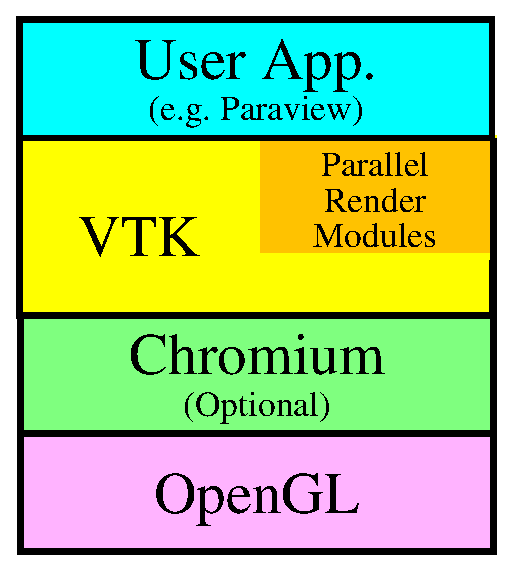
\includegraphics[width=1.5in]{images/AppLayers}
    \caption{A high level view of our proposed visualization system.}
    \label{fig:applayers}
  \end{figure}
  Figure \ref{fig:applayers} shows the layout of the high-level functional
  components of our system.  Rather than build our user level application
  directly on top of a graphical API such as OpenGL, we plan to build our
  applications on top of the VTK framework.  The advantage is twofold: We
  can leverage the enormous visualization code base available with VTK, and
  we can build an application that can be flexible enough to accept
  emerging visualization technologies.  We can also potentially layer VTK
  on top of Chromium to leverage Chromium's powerful parallel rendering
  capabilities.  Because Chromium's interface mimics that of OpenGL, we can
  optionally add or remove that layer with little impact on the system.
  This paper describes our work adding modules to VTK that can
  interchangeably perform various cluster-driven parallel rendering
  algorithms.


  %This figure really belongs to sec:parallel_rendering_interface, but it's
  %moved up so that it resides on the same page as the section.
  \begin{figure*}
    \begin{center}
      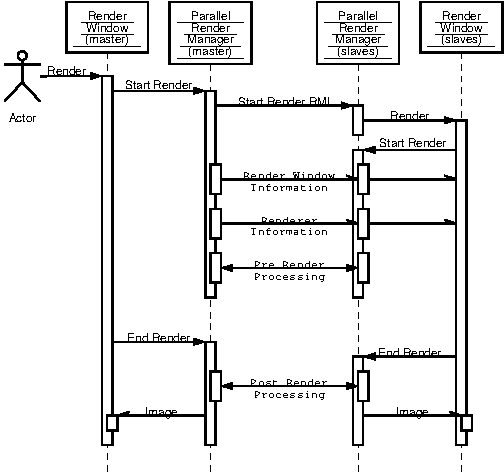
\includegraphics[width=4in]
		      {images/ParallelRenderManagerInteraction}
    \end{center}
    \caption{Interactions of the parallel render manager during render.}
    \label{fig:parallel_render_manager_interaction}
  \end{figure*}


  \section{Previous Work}
  \label{sec:previous_work}

  Thanks to a recent collaboration between Kitware and the ASCI/VIEWS
  program, VTK now supports parallel programming and can be run on cluster
  computers \cite{Ahrens00}.  The parallel VTK libraries support several
  parallel modes.  The mode we concern ourselves with in this paper is data
  parallelism in which the input data is split amongst processes, the
  pieces are filtered and rendered independently, and then composited to
  one image in the end.  This method allows us to make effective use of the
  parallel and distributed nature of our clusters, but can break down if
  the model pieces are too big to be processed by the available
  resources\footnote{Ahrens et al. \cite{Ahrens01} describe using VTK in a
  streaming mode to perform out-of-core processing of data.}.

  While parallel visualization and rendering are now supported by VTK,
  display to a power wall and desktop delivery currently are not.  Instead,
  all current parallel rendering codes in VTK assume that the user
  interface is available at the ``root'' process in a parallel job.  One
  possible approach for driving power walls is to use Chromium
  \cite{Humphreys02}.  Chromium is capable of replacing the OpenGL library
  loaded by an application at runtime, intercepting the stream of OpenGL
  commands, and performing several alterations to it, including driving a
  power wall.  Unfortunately, an OpenGL stream is inherently serial and
  must be issued from a single process, which is a huge bottleneck when
  dealing with large amounts of data.  Chromium also supports a parallel
  rendering mode, but an application must be ``aware'' of Chromium to take
  advantage of this parallel rendering.  We describe our efforts to make
  VTK applications Chromium aware.

  Another power wall display solution available to us is the Image
  Composite Engine for Tiles (ICE-T).  The ICE-T API is an implementation
  of the work presented by Moreland, Wylie, and Pavlakos for efficiently
  performing sort-last parallel rendering onto tile displays
  \cite{Moreland01}.  The ICE-T methodology for rendering fits well with
  VTK's existing parallel rendering paradigm.  We therefore implemented a
  new parallel rendering engine for VTK using the ICE-T API.


  %This figure really belongs to sec:desktop_delivery, but it's moved up so
  %that it resides on the same page as the section.
  \begin{figure*}[ht]
    \begin{center}
      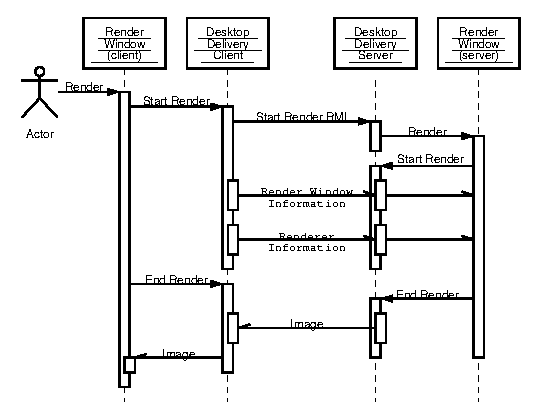
\includegraphics[width=4in]{images/DesktopDeliveryInteraction}
      \caption{Interactions during rendering with desktop delivery.}
      \label{fig:desktop_delivery_interaction}
    \end{center}
  \end{figure*}


  \section{Parallel Rendering Interface}
  \label{sec:parallel_rendering_interface}

  Parallel rendering in VTK is supported via the
  \keyterm{\cidentifier{vtk\-Composite\-Manager}} class.  This class works
  by listening for render events on any renderable VTK window.  After each
  render, but before the images are presented to the user,
  \cidentifier{vtk\-Composite\-Manager} reads back the frame buffers,
  performs a sort-last compositing, and writes the image back to the frame
  buffer.

  Although \cidentifier{vtk\-Composite\-Manager} provides much of the
  functionality we need for our parallel rendering tools, it is
  unnecessarily constrained to a single mode of parallel rendering.  Our
  initial approaches to creating parallel rendering modules involved
  subclassing \cidentifier{vtk\-Composite\-Manager}.  Unfortunately,
  \cidentifier{vtk\-Composite\-Manager} expects its subclasses to only
  handle image data that has already been read from frame buffers.
  Attempting to work around this limitation resulted in obfuscated code.

  Our response was to create a new class,
  \keyterm{\cidentifier{vtk\-Parallel\-Render\-Manager}}.  It works in a
  manner similar to \cidentifier{vtk\-Composite\-Manager} in that they both
  listen to render events and perform appropriate actions around them.  The
  difference is that \cidentifier{vtk\-Parallel\-Render\-Manager} is an
  abstract class designed to give subclasses as much or as little control
  as they need.

  Figure \ref{fig:parallel_render_manager_interaction} outlines how the
  \cidentifier{vtk\-Parallel\-Render\-Manager} behaves during a render
  event.  After the ``master'' or ``root'' parallel render manager receives
  the start render event, it broadcasts a remote method invocation to all
  other parallel render managers to also start a render.  It then
  broadcasts rendering information to all other parallel render managers.
  The parallel render manager also calls protected virtual methods to allow
  subclasses to perform their own data synchronization.  Finally, the
  parallel render manager class calls another protected virtual function to
  allow a subclass to perform any other necessary processing before the
  actual render occurs.

  The \cidentifier{vtk\-Parallel\-Render\-Manager} then relinquishes
  control back to the render window, which proceeds to perform the actual
  image synthesis.  Afterwords, each render window sends an end render
  event to its respective parallel render manager.  The
  \cidentifier{vtk\-Parallel\-Render\-Manager} calls yet another protected
  virtual function to allow subclasses to perform any post-processing, such
  as image composition.

  In addition to handling render events and their propagation and
  synchronization as described above,
  \cidentifier{vtk\-Parallel\-Render\-Manager} also has the following
  features.
  \begin{description}
    \item [Object Creation] Provides factory methods for creating renderer
      and render window objects.  Some parallel rendering schemes require
      fine control over the rendering process.  As such, it may become
      necessary to override the behavior of renderers and render windows.
      By providing object creation, the parallel render manager can help
      ensure the rendering objects match the parallel rendering scheme.
    \item [Boundaries] Will compute the physical boundary, in 3-space, of
      the composite object rendered by all processes.
    \item [Image Reduction] Can reduce the size of the image being rendered
      and then restore the image to full size for viewing.  Reducing the
      image size can drastically reduce the time required for image
      composition strategies.  The class can also automatically set the
      image reduction based on the user's desired rendering rate.
    \item [Image Caching] If the post render processing requires the image
      to be read from the graphics card's frame buffer, the image will be
      cached for potential \cidentifier{vtk\-Parallel\-Render\-Manager}
      users.
  \end{description}

  All of the parallel rendering classes described in this paper inherit
  from \cidentifier{vtk\-Parallel\-Render\-Manager}.  Doing this affords us
  a significant amount of code reuse.  It also provides an abstraction that
  allows us to easily swap the parallel rendering method in our
  applications.

  We have also implemented a class called
  \keyterm{\cidentifier{vtk\-Composite\-Render\-Manager}}.  This class is
  identical in features to the \cidentifier{vtk\-Composite\-Manager} class
  distributed with VTK.  However, having it also inherit from
  \cidentifier{vtk\-Parallel\-Render\-Manager} allows it to play with our
  applications along with our other parallel rendering classes.  The code
  for \cidentifier{vtk\-Composite\-Render\-Manager} is quite small since
  \cidentifier{vtk\-Parallel\-Render\-Manager} does most of the work.  It
  took us very little time to code and debug
  \cidentifier{vtk\-Composite\-Render\-Manager}.  Our goal is to integrate
  these changes into VTK's composite manager.


  \section{Desktop Delivery}
  \label{sec:desktop_delivery}

  Since we in no way expect each analyst to have a parallel cluster
  available in his/her office, we find it important to provide the ability
  of remote desktop delivery.  That is, we wish a user to be able to
  interactively control a visualization job rendering on a cluster and
  display back to a typical desktop machine connected via a local area
  network.

  To this end, we have built a pair of collaborating objects:
  \keyterm{\cidentifier{vtk\-Desktop\-Delivery\-Client}} and
  \keyterm{\cidentifier{vtk\-Desktop\-Delivery\-Server}}.  The client
  object is responsible for accepting user input and displaying rendered
  images.  The server object is responsible for the visualization
  processing and rendering.  The two objects are connected together with a
  pair of \cidentifier{vtk\-Multi\-Process\-Controller} objects.
  \cidentifier{vtk\-Multi\-Process\-Controller}, which is part of the VTK
  distribution, is an abstract interface to parallel process control and
  communication.  The desktop delivery objects expect the process
  controller to control exactly two processes with client and server in
  opposite processes.  The controller used is typically implemented with a
  socket, but does not have to be.

  The \cidentifier{vtk\-Desktop\-Delivery\-Client} object attaches itself
  as an observer to a render window.  When a render event occurs, the
  desktop delivery client object sends a render request to the server along
  with the rendering parameters, waits for an image to come back, and
  pastes the image to the window.  As one would expect, the
  \cidentifier{vtk\-Desktop\-Delivery\-Server} object responds to render
  requests from the client by invoking the render window and shipping the
  resulting image back.  Figure \ref{fig:desktop_delivery_interaction}
  shows the details of this process.

  The reader may notice a striking similarity between the operational
  features of the desktop delivery client/server and the parallel render
  manager described in Section \ref{sec:parallel_rendering_interface}.  In
  particular, the interactions shown in Figures
  \ref{fig:parallel_render_manager_interaction} and
  \ref{fig:desktop_delivery_interaction} are nearly identical.  Because of
  this, both \cidentifier{vtk\-Desktop\-Delivery\-Client} and
  \cidentifier{vtk\-Desktop\-Delivery\-Server} inherit from
  \cidentifier{vtk\-Parallel\-Render\-Manager}.  While this inheritance
  strains the \emph{is-a} requirement dictated by good object-oriented program
  design, we feel the amount of code re-use we achieved was too important
  to neglect.  Furthermore, by inheriting from
  \cidentifier{vtk\-Parallel\-Render\-Manager} we were able to take
  advantage of its boundary calculation and image reduction capabilities,
  both of which are vital properties of our desktop delivery.

  Because the desktop delivery server was designed to enable delivery from
  clusters, it can optionally work with another
  \cidentifier{vtk\-Parallel\-Render\-Manager} object.  The
  \cidentifier{vtk\-Desktop\-Delivery\-Server} performs image delivery
  after the other \cidentifier{vtk\-Parallel\-Render\-Manager} generates
  the image.  The desktop delivery server object uses the other parallel
  render manager to compute the complete object bounds, get timing
  statistics, and otherwise control the parallel rendering process.  The
  desktop delivery server will also take advantage of the other parallel
  render manager's image caching to avoid multiple reads and writes from
  the graphics card frame buffer.


  \section{Chromium}
  \label{sec:chromium}

  We also need to drive power walls in our parallel VTK applications.  One
  means of doing this is with the \keyterm{Chromium} system
  \cite{Humphreys02}.  Chromium intercepts a stream of OpenGL commands and
  filters them.  Chromium's filters are pluggable components called
  \keyterm{stream processing units} (SPUs).  One such unit distributed with
  Chromium is the \keyterm{\cidentifier{tile\-sort}} SPU.  The
  \cidentifier{tile\-sort} SPU determines the area of the screen that
  groups of primitives occupy and ships them to cluster nodes responsible
  for displaying that portion of the screen.

  Because Chromium has the ability to put itself in place of an OpenGL
  shared object library, it can provide a tile display and/or a number of
  other filtering operations to almost any OpenGL application without
  modification or even recompilation.  While flexibility was a major design
  consideration for Chromium, so was efficiency.  As such, many SPUs like
  \cidentifier{tile\-sort} can be applied with little or no degradation of
  frame rates.  However, as mentioned before, using Chromium in serial mode
  is not feasible for large data models, so we must make our application
  Chromium aware so that we can use it in parallel.

  To make our VTK applications Chromium aware, we built the
  \keyterm{\cidentifier{vtk\-Cr\-Render\-Manager}} object.  Because the
  parallel rendering is really being handled by Chromium,
  \cidentifier{vtk\-Cr\-Render\-Manager} does little but allow its
  superclass, \cidentifier{vtk\-Parallel\-Render\-Manager}, to propagate
  render events and parameters.  We also implemented
  \cidentifier{vtk\-Cr\-Open\-GL\-Render\-Window} and
  \cidentifier{vtk\-Cr\-Open\-GL\-Renderer} objects, which the Chromium
  render manager will build for the application.  They work very much like
  their OpenGL counterparts except that they can interface directly with
  the Chromium API.  Currently, they suppress the creation of unused
  windows, provide bounding box hints for \cidentifier{tile\-sort}, and
  provide some interaction with a few other select SPUs.  In time, the
  features of these objects may grow to strengthen the coupling between VTK
  applications and Chromium.

  Using Chromium and its \cidentifier{tile\-sort} SPU, one can achieve very
  impressive frame rates on large power wall displays.  However, this
  approach has scaling issues.  Generally, the number of rendering nodes is
  fixed to the number of tiles being displayed.  Adding more rendering
  nodes requires splitting the tiles into smaller pieces.  This approach
  means the smaller pieces must be recombined to form a full image for each
  tile.  This must be done either with additional image combining hardware
  \cite{Stoll01}, which we don't have, or with software by reading back the
  frame buffer, largely at the expense of frame rates.  Furthermore, the
  sort-first approach to parallel rendering performed by
  \cidentifier{tile\-sort} has inherent scalability and load balancing
  issues.  Some work has been done to correct these issues
  \cite{Samanta99}, but has not yet been implemented in Chromium.

  Of course, Chromium is not bound to the sort-first approach to parallel
  rendering that \cidentifier{tile\-sort} implements.  It can just as
  easily support a sort-last approach, and the \cidentifier{binary\-swap}
  SPU does just that.  Like most sort-last parallel renderers,
  \cidentifier{binary\-swap} scales well with the size of geometry being
  rendered and the number of processors doing the rendering, but at the
  expense of frame rate speeds.  Yet, the sort-last technique is very
  sensitive to the resolution of the output display.  Generating images
  that fit on a typical desktop is feasible, but generating images on high
  resolution tiled displays is not.  We are currently considering
  techniques that may use \cidentifier{tile\-sort} and
  \cidentifier{binary\-swap} to better distribute the work for large
  amounts of data on tiled displays.

%%   Because Chromium is a pluggable architecture supporting both sort-first
%%   and sort-last parallel rendering algorithms, it is conceivable to use a
%%   combination of both.  So another alternative currently available in
%%   Chromium is to assign multiple processes to each tile and use a
%%   \cidentifier{binary\-swap} SPU to generate a single image per tile.
%%   Clients could then use the \cidentifier{tile\-sort} SPU to send
%%   primitives to one processor for each tile.  An example configuration is
%%   shown in Figure \ref{fig:crazy_chromium_crapp}.  While such a setup
%%   should enable larger clusters to realize faster rendering rates, it still
%%   suffers from the same load balancing issues discussed above.
%%   Furthermore, because each polygon must still be pushed onto the wire, we
%%   still expect scalability issues with large amounts of geometry.


  \section{ICE-T}
  \label{sec:ICE-T}

  Another power wall display solution available to us is the \keyterm{Image
  Composite Engine for Tiles} (ICE-T).  The ICE-T API allows applications
  to easily perform sort-last parallel rendering.  It uses several image
  space reduction and compression techniques to make the composition of
  even high resolution tiled displays feasible.  The details of ICE-T's
  algorithms can be found in \cite{Moreland01}.

  Our initial goal was to embed ICE-T into a Chromium SPU.  However, we
  quickly found that this was an impractical target.  The Chromium SPUs,
  because they operate on streams of OpenGL commands, use a \emph{push}
  model.  That is, the application pushes OpenGL commands to the first SPU,
  which pushes them to the next SPU, and so on.  A SPU generally processes
  one command and then moves on.  In contrast, ICE-T uses a \emph{pull}
  model.  ICE-T can perform compositions for images that can be much larger
  than what the available graphics card can render in one pass.  It
  therefore may have to pull several images of the same geometry rendered
  with different projections.  For this to be performed in a Chromium SPU,
  the entire OpenGL stream would have to be cached each frame.  This would
  be very inefficient for large amounts of geometry, which ICE-T was
  specifically designed to handle.  We briefly considered Chromium hints
  and extensions that might make the application's data available.
  Ultimately, we decided that trying to shoehorn ICE-T into Chromium like
  this would require applications to be so tailored to the ICE-T SPU that
  they might as well use the ICE-T API directly.

  We were able to instead embed ICE-T into the VTK framework.  We found
  this much more practical because, like ICE-T, VTK uses a \emph{pull}
  model.  A render request is given to the window at the bottom of the VTK
  pipeline.  The event is propagated up the pipeline as each component
  pulls fresh geometry or images from the component above it.  ICE-T fits
  well in this framework.

  To start, we built an object called
  \keyterm{\cidentifier{vtk\-Ice\-T\-Render\-Manager}}.  As always, this
  class inherits from \cidentifier{vtk\-Parallel\-Render\-Manager}.  As
  such, it attaches itself to a render window and listens for render
  events.  \cidentifier{vtk\-Ice\-T\-Render\-Manager} works in conjunction
  with the ICE-T API to compose images.

  However, ICE-T also must in some cases transform the projection matrix
  and perform several renderings.  This behavior is beyond that of a
  \cidentifier{vtk\-Parallel\-Render\-Manager} unit, so we designed an
  object called \cidentifier{vtk\-Ice\-T\-Renderer} to handle this.
  \keyterm{\cidentifier{vtk\-Ice\-T\-Renderer}} responds to ICE-T render
  requests and returns the appropriate images.  The ICE-T render manager
  object will create ICE-T renderer objects for the user level application.

  The ICE-T render manager also builds on the concept of image reduction.
  Unlike the image reduction of the parent
  \cidentifier{vtk\-Parallel\-Render\-Manager} class, the ICE-T render
  manager does not reduce the size of the renderable viewport.  Recall that
  in a tiled display, the overall display size is larger than any one
  image.  ICE-T uses an extension of the \emph{floating viewport} described
  in Moreland, Wylie, and Pavlakos \cite{Moreland01} to render images
  spanning multiple tiles and therefore reduce the number of times the
  geometry must be rendered.


  \section{Steering Station}
  \label{sec:steering_station}

  Another important issue with rendering to tiled displays is providing an
  interface with which users can interact.  The typical solution for VTK
  applications using a composite manager such as ParaView is to place the
  user interface at node 0 where the image is displayed \cite{Law01}.  This
  is problematic with a tile display for several reasons.  The most
  significant problem for us is the fact that, for security reasons, our
  display wall and driving cluster are in different rooms, separated by a
  bolted steel door.  Instead, our user interface resides on a
  \keyterm{steering station,} a separate PC located in view of the display
  and connected to the cluster via a standard Ethernet connection.  Changes
  made in the user interface running on the steering station are then
  propagated to the images on the display wall.

  It so happens that this exact functionality is already implemented by the
  desktop delivery objects described in Section \ref{sec:desktop_delivery}
  except that images are displayed on the server rather than shipped back
  the client.  Therefore, the desktop delivery server object has a flag to
  select the display.  If displaying to the client, the behavior is as
  described in Section \ref{sec:desktop_delivery}.  If displaying to the
  server, the render windows on the server side are never resized and
  images are not transferred back to the client.  The client simply renders
  a very coarse representation of the geometry, which is a bounding box by
  default.


  \begin{figure}
    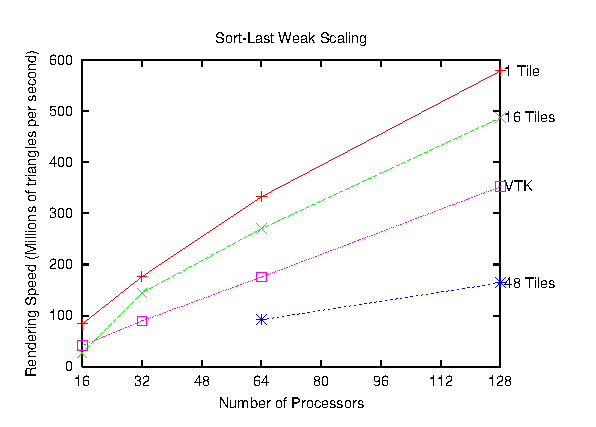
\includegraphics[width=\linewidth]{images/scaling_icet_weak}
    \caption{Scaling of sort last parallel rendering.  ICE-T is used to
      render to various tile layouts.  The performance of the compositor
      distributed with VTK is also measured.  Each application processor
      renders about 7.4 million triangles (i.e. larger jobs have more
      triangles).}
    \label{fig:ice-t}
  \end{figure}

  \begin{figure}
    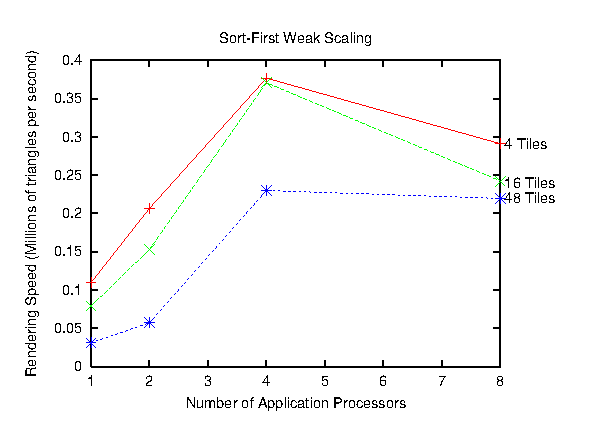
\includegraphics[width=\linewidth]{images/scaling_chromium}
    \caption{Scaling of parallel rendering using Chromium's
      \cidentifier{tile\-sort} SPU.  Each client renders about 7.4 million
      triangles (i.e. larger jobs have more triangles).  Measurements were
      taken using a 100BaseT network.}
    \label{fig:chromium}
  \end{figure}

  \section{Conclusion}
  \label{sec:conclusion}

  With the introduction of the desktop delivery, Chromium, and ICE-T
  components into VTK, we have shown that VTK is a viable framework for
  cluster-based interactive applications that require remote display or
  display to high-resolution power walls.  By using both the image-centric
  level of detail provided by the reduction factors in conjunction with the
  geometry-centric level of detail directly provided by VTK, we can achieve
  highly interactive rendering for almost any image transfer, compositing,
  or rendering speeds.  \sticky{Some empirical evidence, i.e. with LLNL
  data, would probably be good here.  But how?  You really need a video and
  see it in action.}

%%   \begin{figure}
%% %%     \includegraphics[width=\linewidth,viewport=.75in .75in 10.25in 7.75in]
%% %% 		    {images/scaling}
%%     \includegraphics[width=\linewidth,bb=60 76 725 537]
%% 		    {images/scaling}
%%     \caption{Comparison of rendering times using sort-last and sort-first
%%       parallel rendering.}
%%     \label{fig:scaling}
%%   \end{figure}

%%   A comparison between a sort-first approach like Chromium's
%%   \cidentifier{tile\-sort} SPU and a sort-last approach like ICE-T reveals
%%   very different rendering characteristics.  Figure \ref{fig:scaling} shows
%%   the rendering performance of ICE-T for various sizes of input geometry
%%   and the theoretical maxium performance of Chromium\footnote{Initial
%%   experiments indicate that clients are running at low network efficiencies
%%   (on the order of 12-14\% of theoretical peak shown in \ref{fig:scaling}),
%%   which we suspect are due to buffer size and flow control issues in
%%   Chromium's GM implementation. We are investigating the issue and hope to
%%   have scaling benchmarks by the time of the conference.}.  The timings are
%%   taken from a job that runs on 32 processors and displays on 9 tiles, each
%%   having a resolution of $1280 \times 1024$ pixels.  When the input
%%   geometry is relatively small, Chromium's \cidentifier{tile\-sort} can
%%   generate real time frame rates of 30~Hz or better, while ICE-T's
%%   sort-last approach can barely run over 5~Hz.  However, when the input
%%   geometry is larger than 20 million polygons, the overhead of compositing
%%   images in the sort-last approach becomes smaller than the overhead of
%%   transferring polygons in the sort-first approach.  Therefore, in this
%%   case the sort-last approach can achieve faster rendering rates, albeit at
%%   quite low frame rates.

%%   \sticky{Comparison of rendering times of Chromium and ICE-T for various
%%   geometry sizes.  I would have it here already, but after a month I still
%%   don't have the Chromium stuff working on our cluster.  It's driving me
%%   nucking futs.}

  Our ability to abstractly swap the parallel rendering method is of
  tremendous importance.  Each method of parallel rendering has its own
  strengths and weaknesses, and it may be imperative to pick the method
  that best fits the current usage for the system.  For example, when using
  our sort last methods on our cluster (comprised of 128 Dell Precision 530
  workstations, each with dual 2.0 GHz Pentium-4 Xeon CPUs, 1 GB RDRAM, a
  GeForce 3 graphics card, and interconnected with Myrinet 2000), we find
  that even with very little geometry we can achieve frame rates of only
  about 10~Hz for our tile displays due to the overhead of image
  compositing.  However, as can be seen in Figure \ref{fig:ice-t}, with
  sufficiently large input geometry we can achieve very impressive
  rendering performance even on tiled displays.

  In contrast, the Chromium \cidentifier{tile\-sort} SPU has been shown to
  be able to render with frame rates in excess of 40~Hz \cite{Humphreys02}.
  However, our current method of rendering has the number of Chromium
  ``server'' nodes fixed to the number of tiles and we see from Figure
  \ref{fig:chromium} that we get negative returns attempting to use more
  than about four application processes.  Thus, we can only use our current
  Chromium configuration with modest sized data.  It is conceivable to
  build other Chromium configurations that allow for better rendering
  performance of large data on tile displays, but race conditions existing
  in the Chromium network layer at the time of this writing have prohibited
  us from experimenting in this arena.  These race conditions have also
  prohibited us from showing the scaling behavior past eight application
  processors in Figure \ref{fig:chromium}.

%%   One drawback of the ICE-T composite objects is that they only work with
%%   OpenGL rendering and MPI communications.  This is because, due to
%%   historical reasons, the ICE-T API is dependent on the OpenGL and MPI
%%   APIs.  In retrospect, coupling the compositing API with any particular
%%   rendering or communications API was not beneficial.  Nevertheless, OpenGL
%%   and MPI remain the \emph{de facto} standards.


  \section{Future Work}
  \label{sec:future_work}

  We have just begun the process of creating a viable production-quality
  tool to run on our clusters and display on our power walls.  There is
  much work still to be done.

  Our desktop delivery objects allow for any type of interface to be built
  on the client side.  However, we currently have not built a GUI capable
  of much more than simple navigation controls.  Ultimately, we would like
  a fully-featured visualization tool such as \keyterm{ParaView}
  \cite{Law01} to be presented at the desktop.  We currently have a
  contract with Kitware (\href{http://www.kitware.com}{www.kitware.com}) to
  incorporate the technologies described in this paper into ParaView.  The
  latest version of ParaView is available free from
  \href{http://www.paraview.org}{www.paraview.org}.

  The two methods of rendering to tile walls discussed have diametrical
  performance properties.  Chromium's \cidentifier{tile\-sort} excels at
  providing fast frame rates for small amounts of geometry while ICE-T
  excels at rendering large amounts of geometry.  We would like our
  application to be able to pick the most appropriate rendering method.
  Unfortunately, Chromium and ICE-T have to be launched in different ways.
  An application cannot easily switch between the two.  Our proposed
  solution is to instead modify ICE-T to take advantage of data
  replication.  By replicating the geometric data we can reduce the amount
  of image data that needs to be processed and can thereby greatly increase
  the speed of image composition.

  While the concept of a steering station allows an arbitrarily complex
  user interface, it can be less than ideal.  Often, we find the user
  walking to the wall for a closer look and back to the steering station to
  drive the application.  We would like to incorporate a hand-held device
  that could move with the user and at least provide navigation controls.


  \section{Acknowledgments}

  This work was performed at Sandia National Laboratories.  Sandia is a
  multi-program laboratory operated by Sandia Corporation, a Lockheed
  Martin Company, for the United States Department of Energy under contract
  DE-AC04-94AL85000.

  We would also like to give a special thanks to Brian Wylie for his
  support, inspiration, and the encouragement to write this paper in the
  first place.


  \bibliographystyle{acmsiggraph}
  \bibliography{vtkicet}

  \begin{figure*}[!p]
    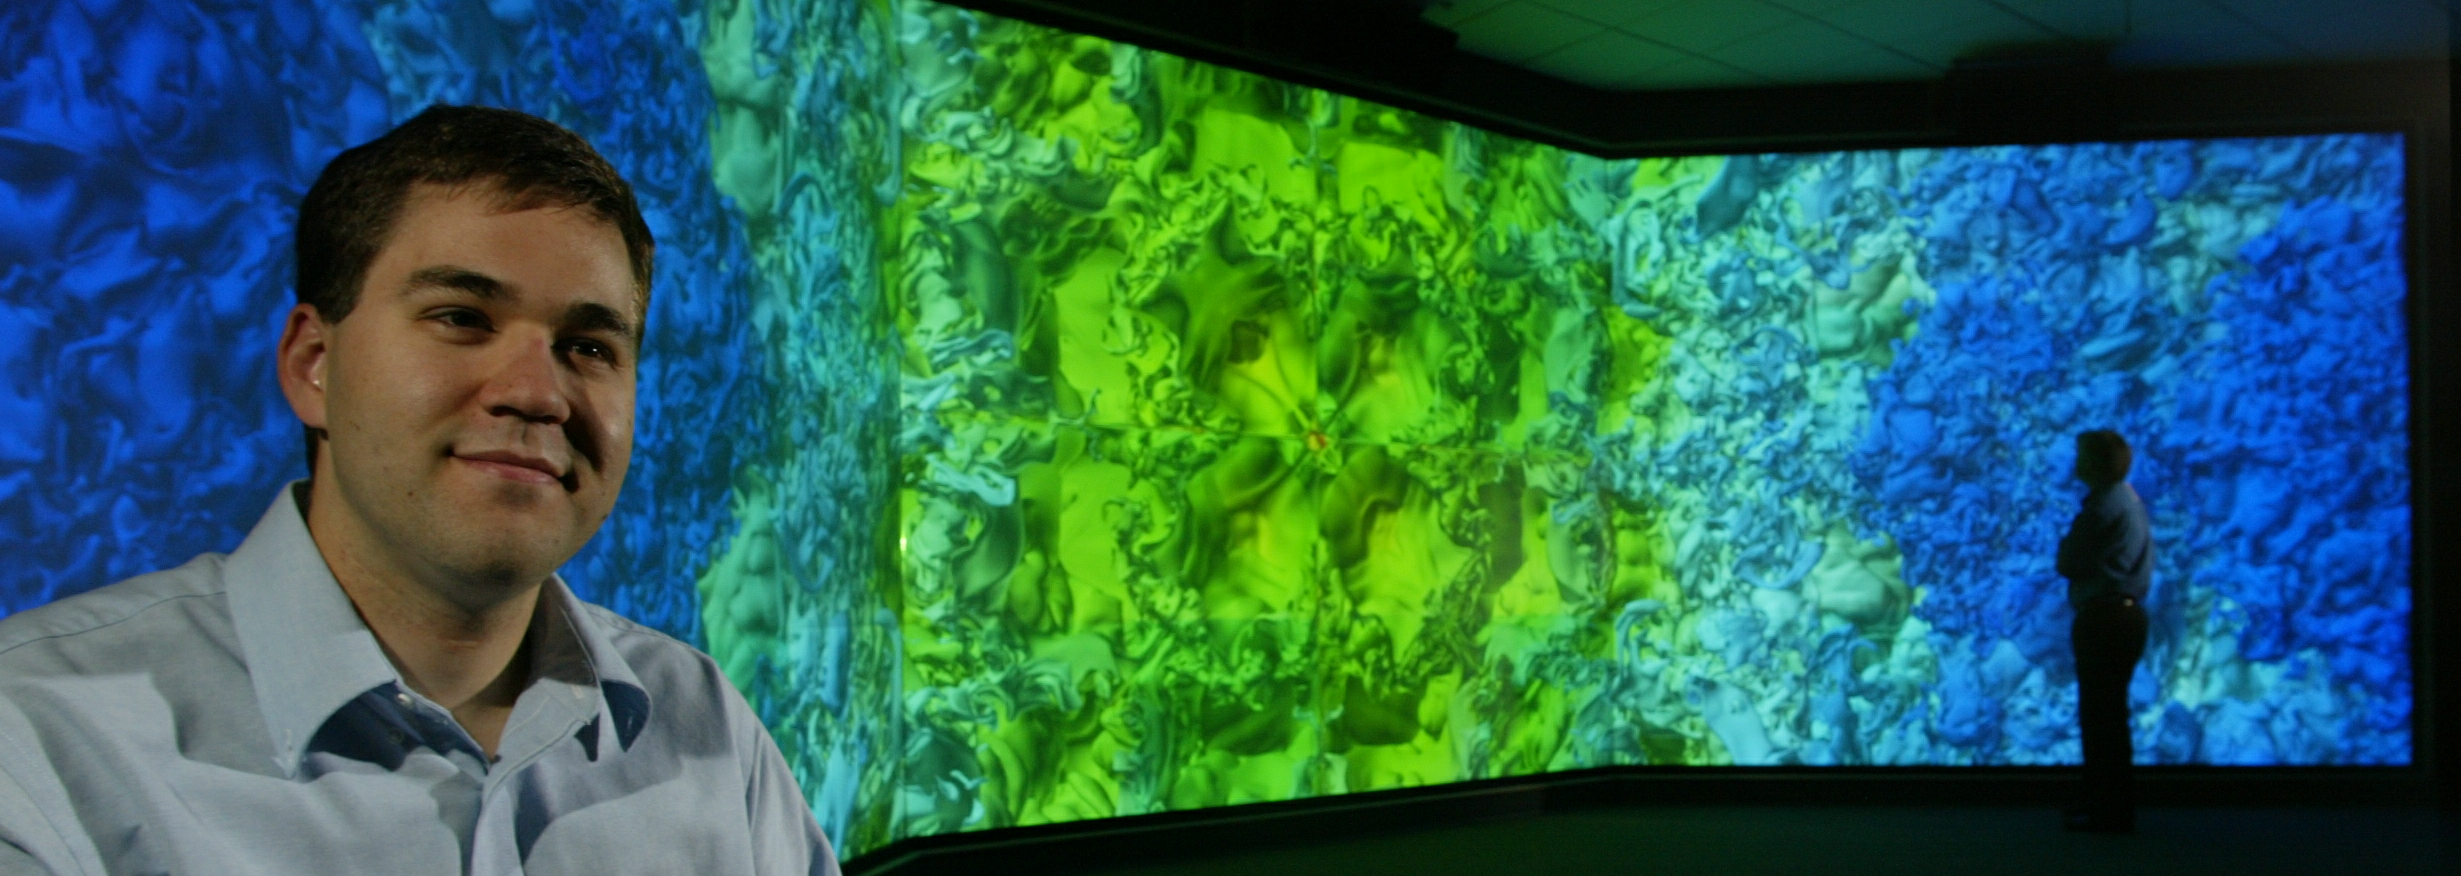
\includegraphics[width=\textwidth]{images/FullWall}
    \caption{The VIEWS Corridor display.  The display contains about 63
    million pixels.  The isosurface being displayed contains about 470
    million triangles.  Our VTK application can render this isosurface on
    our display in about 15 seconds.  With coarser levels of both geometric
    and image detail, we can sustain a minimum frame rate of 5--10~Hz.
    \sticky{Might want to verify that.}}
    \label{fig:fullwall}
  \end{figure*}

  \begin{figure*}[!p]
    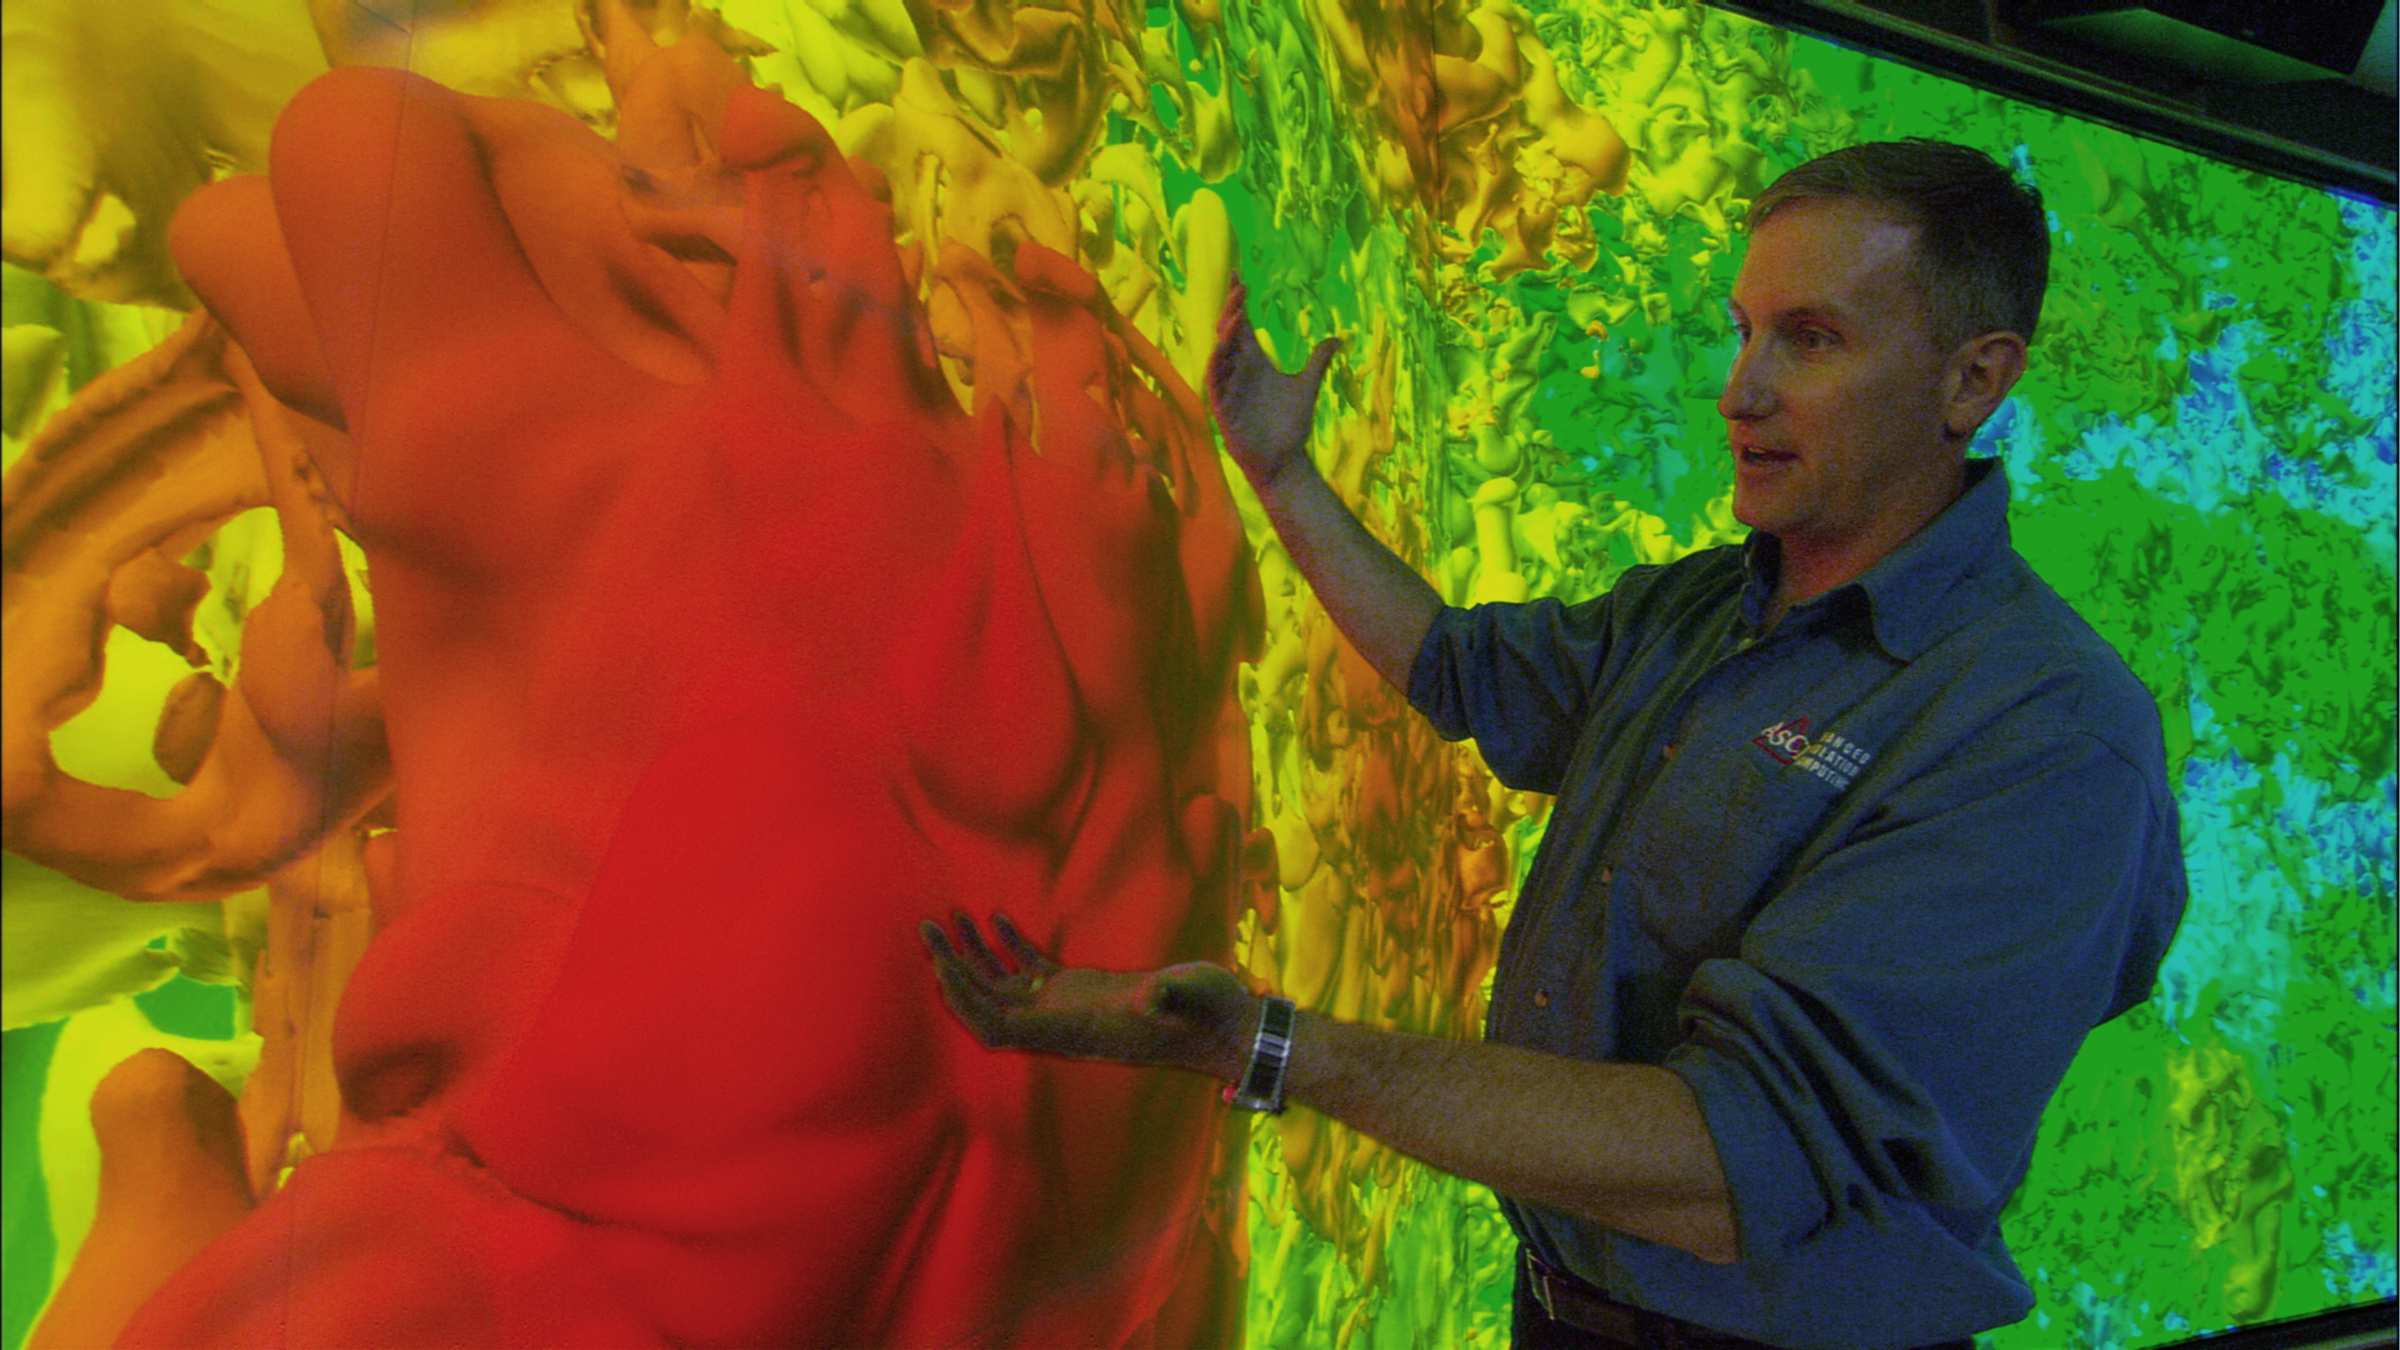
\includegraphics[width=\textwidth]{images/PhilwBlob}
    \caption{Our manager, Philip Heermann, inspecting a plume of gas.
    Philip can inspect the details of the plume without losing the context
    of the rest of the model.}
    \label{fig:philwblob}
  \end{figure*}

\end{document}
